\chapter{Especificações técnicas e arquitetura}

\section{Flutter}
O aplicativo foi desenvolvido utilizando o SDK de desenvolvimento Flutter. Flutter é um conjunto de ferramentas de código aberto desenvolvido pelo Google. Sua primeira versão foi lançada em 2018. O objetivo do Flutter é permitir a criação de aplicativos Android e iOS onde o resultado seja equivalente a um aplicativo desenvolvido nativamente mas com uma base de código em comum para as duas plataformas. O SDK utiliza internamente a biblioteca gráfica Skia para renderizar o aplicativo.

\section{Dart}
Dart é a linguagem de programação utilizada em Flutter. Dart é uma linguagem desenvolvida e otimizada para se desenvolver interfaces de usuário interativas. A linguagem compila para ARM e código de máquina x64, que são as arquiteturas mais utilizadas atualmente. Também é possível compilar Dart para Javascript e utilizá-lo na Web. É possível compilar Dart de duas formas: \textit{Ahead of Time} (AOT) e \textit{Just in Time} (JIT). Utiliza-se AOT ao gerar o código que irá rodar em produção pois ele contém mais verificações e bloqueia a compilação em tempo de execução. já para código em desenvolvimento utiliza-se JIT, o que permite um ciclo de desenvolvimento mais ágil já que nem toda a aplicação precisa ser reconstruída de uma vez só. Devido a essa flexibilidade, é possível utilizar a técnica chamada de \textit{Hot reload} ou carregamento quente (tradução livre) onde o desenvolvedor pode modificar apenas um arquivo e quase instantaneamente verificar o resultado na aplicação.

\section{Arquitetura}
Comumente em desenvolvimento \textit{mobile}, como por exemplo no Android SDK ou iOS UIKit, o desenvolvimento acontece de forma imperativa, ou seja, aquilo que o usuário está vendo em determinado momento é definido a partir de uma sequencia de instruções dadas pelo desenvolvedor. Já em Flutter a aplicação é desenvolvida de forma declarativa, portanto aquilo que o usuário ve não é construído a partir de uma sequencia de instruções, em vez disso representa um estado que pode ser representado por uma variável, uma estrutura de dados ou uma classe.

Se há uma mudança no estado da aplicação o \textit{framework} atualiza a interface de usuário e redesenha todos os componentes para representar o estado atual. Não é possível acessar um único componente e modificá-lo diretamente, em vez disso é necessário atualizar o estado da aplicação. Devido a essa natureza declarativa, gerenciamento de estados é um fator importante no desenvolvimento em Flutter.

Há várias bibliotecas e arquiteturas para facilitar esse processo, algumas delas especificas para Flutter, por exemplo: Provider, BLoC e Redux. O método utilizado nesse projeto é uma mistura de BLoC com Redux. BLoC ou \textit{Business Logic Component} (Componente de lógica de negócios) baseia-se em separar o código de interface de usuário da lógica de negócios. 


Redux é um \textit{framework} desenvolvido por Dan Abramov primeiramente para desenvolvimento web e eventualmente adaptado para outras plataformas. Geralmente Redux é apresentado como um container de estados previsíveis, na prática isso significa uma maneira de gerenciar a interface de usuário da aplicação a partir de um estado global. Neste projeto o estado é construído na camada de lógica de negócios e os \textit{Widgets} do flutter reagem a qualquer mudança que ocorra no objeto de estado. Uma visão geral da arquitetura do projeto pode ser vista nas figuras 5 e 6 a seguir:

\begin{figure}[H]
	\caption{\label{fig:bloc_flow}Figura 5 - BLoC Flow}
	\begin{center}
		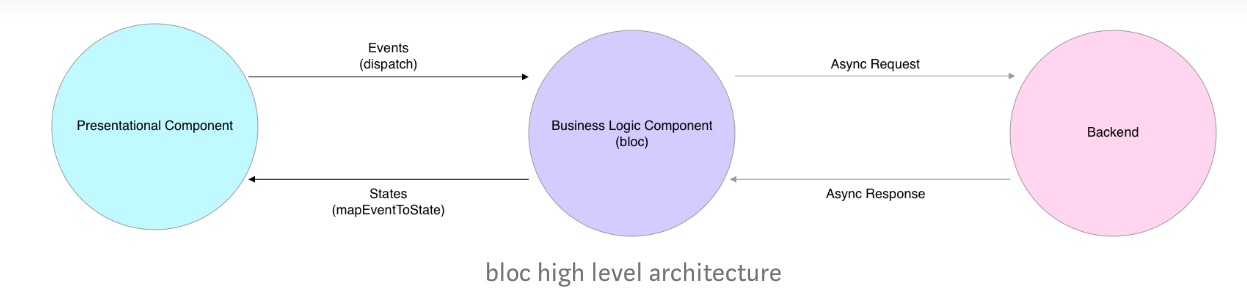
\includegraphics[scale=0.50]{bloc_flow}
	\end{center}
	%\legend{Fonte: \citeauthor{ihs2013}, \citeyear{ihs2013} (Adaptado)}
\end{figure}



\begin{figure}[H]
	\caption{\label{fig:arquitetura_tozzi}Figura 6 - Arquitetura Tozzi}
	\begin{center}
		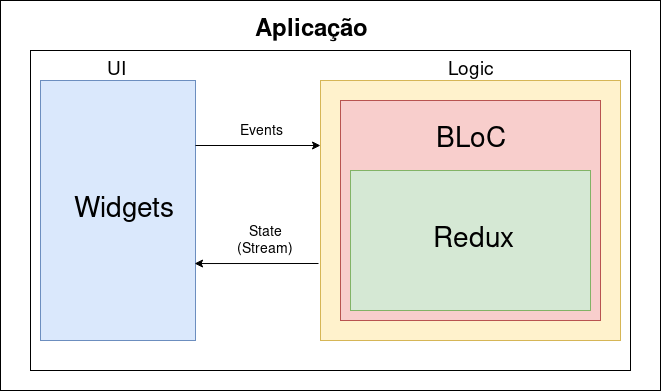
\includegraphics[scale=0.50]{arquitetura_tozzi}
	\end{center}
\legend{Fonte:Disponível em: . Acesso em: 30 set. 2019.}
\end{figure}

Sempre que o usuário interagir com o aplicativo, essa interação emite eventos a partir da camada de UI através dos Widgets para a camada de lógica onde o Redux mapeia esse evento para um possível estado da aplicação. A camada de interface escuta por mudanças no estado e renderiza novamente quando há uma variação no estado.

\begin{figure}[htb]
	\caption{\label{fig:redux}Figura 7 - Redux Tozzi}
	\begin{center}
		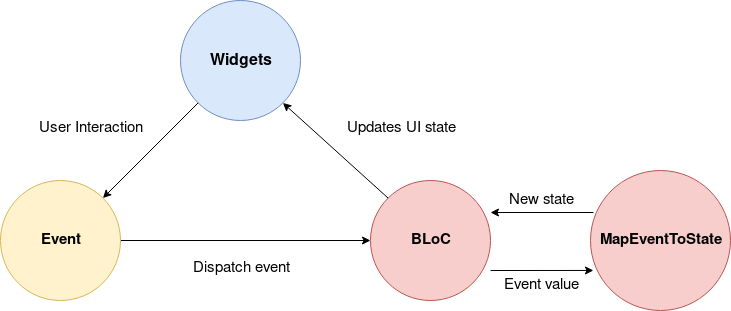
\includegraphics[scale=0.79]{redux_tozzi}
	\end{center}
	%\legend{Fonte: \citeauthor{ihs2013}, \citeyear{ihs2013} (Adaptado)}
\end{figure}





\section{Backend}
Foi desenvolvido um \textit{backend} para a aplicação com o objetivo de gerenciar os dados e as sesssões de usuário. Utilizou-se ASP.NET Core para desenvolver uma RESTful API. .NET Core é a reimplementação de código aberto da plataforma .NET Framework criada pela Microsoft. ASP.NET Core é uma boa opção para o desenvolvimento de aplicações \textit{backend} pois é eficiente, altamente escalável e rápido. De acordo com testes efetuados pela empresa \textit{TechEmpower} ASP.NET Core está entre as aplicações para \textit{WebAPI} mais eficientes. Aplicações desenvolvidas com ASP.NET Core também podem utilizar o serviço de hospedamento Azure da Microsoft gratuitamente. 

PostgreSQL foi o banco de dados utilizado no desenvolvimento da aplicação. PostgreSQL é um banco de dados relacional de código aberto que utiliza linguagem SQL para operar em dados, funciona na maioria dos sistemas operacionais atualmente e segue todas as convenções de banco de dados, sendo as mesmas: atomicidade, consistência, isolação e durabilidade.

